\documentclass[
    10pt,
    aspectratio=169,
]{beamer}
\usepackage{transparent}
\usepackage{booktabs} 
\usepackage{tabularx}
\usepackage{makecell}
\beamertemplatenavigationsymbolsempty
%\usepackage{appendixnumberbeamer} %If you want a separate slide counter for your appendix
\usepackage{tikz}
\usepackage{colortbl}
%%% To add citations
\usepackage[
    style=nature,
    sorting=none,
    isbn=false,
    url=false,
    doi=true,
    eprint=false,
    date=year,
    maxnames=3,
    minnames=2
]{biblatex}
\addbibresource{bibliography.bib}
\renewcommand*{\bibfont}{\normalfont\fontsize{5}{5}\selectfont}
\usepackage{algorithm}
\usepackage{algpseudocode}
\usepackage{lipsum}
\usepackage{hyperref}
%%% Customize Theme %%%%%%%%%%%%%%%%%%%%%%
\usetheme[width=3.8em]{boxes} %Beamer themes here https://deic.uab.cat/~iblanes/beamer_gallery/index_by_theme.html


% \addtobeamertemplate{sidebar right}{}{ 
%  \hspace*{.5em}{\transparent{0.5} \includegraphics[width = 0.131\textwidth]{University_of_Southern_California_seal.svg.png}}%
% }

%----------------------------------------------------------
%           Colour Setup
%----------------------------------------------------------

%fg = font color
%bg = background color

% ! WARNING ! : Many colors are linked to multiple attributes, so changing one color can have unexpected changes!

% If you want to tweak the shading of orange and red, tweak the below 2 lines:
\definecolor{myRed}{RGB}{163, 10, 53}
\definecolor{myOrange}{RGB}{254, 190, 16}
\definecolor{tableGreen}{HTML}{90EE90}
\definecolor{tableOrange}{HTML}{FFD700}

\setbeamertemplate{sidebar canvas right}[vertical shading][top=myRed, middle=myRed!85, bottom=myRed]
% Bottom right hand color
\setbeamercolor*{structure}{bg=myOrange,fg=myRed}

\setbeamercolor*{palette primary}{use=structure,fg=white,bg=structure.fg} %?
\setbeamercolor*{palette secondary}{use=structure,fg=myRed,bg=myOrange}
    %bottom left of footer & bar between title & top bubbles
\setbeamercolor*{palette tertiary}{use=structure,fg=white,bg=myRed} 

\setbeamercolor{frametitle}{bg=myRed,fg=white} %title of each slide

\setbeamercolor*{titlelike}{parent=palette primary} %?



%%% Edits ONLY the TOC slide %%%
\setbeamercolor{section in toc}{fg=black}
\setbeamercolor{subsection in toc}{fg=black}

%%% Block Colors %%%
% Standard block %
    \setbeamercolor{block title}{bg=myOrange, fg=white}
    \setbeamercolor{block body}{bg=myOrange!20}

% Alerted block % If you want to customize it's color
    %\setbeamercolor{block title alerted}{bg=cyan, fg=white}
    %\setbeamercolor{block body alerted}{bg=cyan!10}

% Example block % If you want to customize it's color
    %\setbeamercolor{block title example}{bg=cyan, fg=white}
    %\setbeamercolor{block body example}{bg=cyan!10}

\setbeamercolor{title in sidebar}{fg=white!75}
\setbeamercolor{author in sidebar}{fg=white!50}
\setbeamercolor{palette sidebar secondary}{fg=myRed,bg=white!80}
\setbeamercolor{subsection in sidebar}{fg=myRed,bg=white!80}
\setbeamercolor{section in sidebar shaded}{fg=white!75}
\setbeamercolor{subsection in sidebar shaded}{fg=white!75}
%---------------------------------------------------------
%	SELECT FONT THEME & FONTS
%---------------------------------------------------------

\usefonttheme{serif}
\usepackage{fontenc}
\usepackage{ebgaramond}

\setbeamerfont{frametitle}{size=\large}

%---------------------------------------------------------
%	SELECT OUTER THEME
%---------------------------------------------------------
% Outer themes change the overall layout of slides, such as: header and footer lines, sidebars and slide titles. Uncomment each theme in turn to see what changes it makes to your presentation.

\useoutertheme{default}

% This sets up the footer on each slide

\setbeamercolor{section in foot}{fg=white, bg=myRed}


\setbeamertemplate{footline}
{
 \hbox{%
  \begin{beamercolorbox}[wd=.12\paperwidth,ht=2.6ex,dp=2ex,center]{section in foot}%
    \usebeamerfont{section in foot}\insertshortauthor
  \end{beamercolorbox}%
  
  \begin{beamercolorbox}[wd=.65\paperwidth,ht=2.6ex,dp=2ex,center]{section in foot}%
    \usebeamerfont{section in foot} \insertshorttitle \hspace{1em} \insertframenumber/\inserttotalframenumber
  \end{beamercolorbox}%
  
  \begin{beamercolorbox}[wd=.2\paperwidth,ht=2.6ex,dp=2ex,center]{section in foot}%
    \usebeamerfont{section in foot} 
  \end{beamercolorbox}}%

  \vskip0pt%
}



% Other Frames to consider...

%\useoutertheme{miniframes}
%\useoutertheme{infolines}
%\useoutertheme{smoothbars}
%\useoutertheme{sidebar}
%\useoutertheme{split}
%\useoutertheme{shadow}
%\useoutertheme{tree}
%\useoutertheme{smoothtree}

%---------------------------------------------------------
%	PRESENTATION INFORMATION
%---------------------------------------------------------

\title[Short Title]{Your Presentation Title Here}
%\subtitle{Optional Subtitle}
\author[Initials]{Your Name Here}

\date{\today}
\institute[Institution]{Your Department or Institute \\
Your University Name }

%%% This sets up the title page

\titlegraphic{
  \begin{tikzpicture}[remember picture, overlay]
    % 
    \node[anchor=south west, xshift=0cm, yshift=0.5cm] at (current page.south west) {
      
\includegraphics[height=1cm]{logos/USC_seal.png}
    };

    % 
    \node[anchor=south east, xshift=-0.5cm, yshift=0.5cm] at (current page.south east) {
      
\includegraphics[height=1cm]{logos/isi.png}
    };
    
    % % 
    % \node[anchor=north east, xshift=-0.8cm, yshift=-0.3cm] at (current page.north east) {
    %   \includegraphics[height=1.1cm]{logos/CleanEasy-logo3.png}
    % };
    
    % %
    % \node[anchor=north east, xshift=-2.8cm, yshift=-0.3cm] at (current page.north east) {
    %   \includegraphics[height=1.4cm]{logos/CleanEasy-logo4.png}
    % };
  \end{tikzpicture}
}
% \setbeamertemplate{title page}{
%   \begin{minipage}[b][\paperheight]{\textwidth}
%     \vfill%
%     \ifx\inserttitle\@empty\else\usebeamertemplate*{title}\fi
%     \ifx\insertsubtitle\@empty\else\usebeamertemplate*{subtitle}\fi
%     \usebeamertemplate*{title separator}
%     \ifx\beamer@shortauthor\@empty\else\usebeamertemplate*{author}\fi
%     \ifx\insertdate\@empty\else\usebeamertemplate*{date}\fi
%     \ifx\insertinstitute\@empty\else\usebeamertemplate*{institute}\fi
%     \vfill
%     \vspace*{1mm}
%   \end{minipage}
%     \raisebox{.1\paperheight}[1.7em][0em]{%
%     \makebox[\paperwidth][c]{%
%       \hspace*{-8.2em}\includegraphics[width=.883\paperwidth,height=1cm]{PHP.png}%
%     }%
%   }
% }
\makeatother

%---------------------------------------------------------
%---------------------------------------------------------
%---------------------------------------------------------
\begin{document}

%---------------------------------------------------------
%	TITLE SLIDE
%---------------------------------------------------------
\section{}
\begin{frame}
	\titlepage % Output the title slide, automatically created using the text entered 
\end{frame}

%---------------------------------------------------------
%	TABLE OF CONTENTS SLIDE
%---------------------------------------------------------
% References sections and subsections, specified with the standard \section and \subsection commands. If you want to display all sections and subsections on one slide, just use \tableofcontents. If you want to just display each section one at a time (in subsequent slides) use \tableofcontents[pausesections].

%\tableofcontents



%---------------------------------------------------------
%	PRESENTATION BODY SLIDES
%---------------------------------------------------------

%==========================================================
% SECTION 1: INTRODUCTION & METHODS
%==========================================================

% \section{Introduction}
\begin{frame}{Introduction}
\begin{itemize}
    \item First key point introducing your topic and providing context
    \item Second point explaining the problem or research question you're addressing
    \item Third point describing why this work is important or relevant
    \item Fourth point outlining your approach or main contribution
\end{itemize}
\end{frame}

\begin{frame}{Dataset}
\begin{itemize}
    \item \textbf{Data Source:} Description of where your data comes from
    \begin{itemize}
        \item Key characteristic one of the data
        \item Key characteristic two of the data
        \item Key characteristic three of the data
    \end{itemize}
    \item \textbf{Target Variable:} What you are predicting or analyzing
    \begin{itemize}
        \item Why this target was selected
        \item Definition or classification scheme
    \end{itemize}
    \item \textbf{Dataset Composition:}
    \begin{itemize}
        \item Total number of samples and their distribution
        \item Sampling strategy or selection criteria
        \item Class balance or distribution information
        \item Train/test/validation split ratios
    \end{itemize}
    \item \textbf{Preprocessing:} Description of data cleaning and preparation steps
\end{itemize}
\end{frame}

\begin{frame}{Methods Overview}
\begin{itemize}
    \item Description of your methodological approach:
    \begin{itemize}
        \item \textbf{Method 1} - Brief description and key parameters
        \item \textbf{Method 2} - Brief description and key parameters
        \item \textbf{Method 3} - Brief description and key parameters
    \end{itemize}
\end{itemize}
\end{frame}

\begin{frame}{Approaches Tested: Example Multi-Column Layout}
\small
\begin{columns}[t]
\column{0.5\textwidth}
\textbf{Category A Approaches (X total)}
\begin{itemize}
  \item \textbf{Subcategory 1 (N):} Approach A, Approach B, Approach C
  \item \textbf{Subcategory 2 (N):} Approach D, Approach E
  \item \textbf{Subcategory 3 (N):} Approach F, Approach G, Approach H
  \item \textbf{Subcategory 4 (N):} Approach I, Approach J, Approach K
  \item \textbf{Subcategory 5 (N):} Approach L
\end{itemize}

\column{0.5\textwidth}
\textbf{Category B Approaches (Y total)}
\begin{itemize}
  \item \textbf{Variant 1 (N):}
  \begin{itemize}
    \scriptsize
    \item Method A, Method B, Method C, Method D, Method E
  \end{itemize}
  \item \textbf{Variant 2 (N):}
  \begin{itemize}
    \scriptsize
    \item Method F, Method G, Method H, Method I, Method J
  \end{itemize}
  \item \textbf{Variant 3 (N):}
  \begin{itemize}
    \scriptsize
    \item Method K, Method L, Method M, Method N, Method O
  \end{itemize}
  \item \textbf{Variant 4 (N):}
  \begin{itemize}
    \scriptsize
    \item Method P, Method Q, Method R, Method S, Method T
  \end{itemize}
\end{itemize}
\end{columns}
\end{frame}

%   \item \textbf{Notes:}
%     \begin{itemize}
%       \item \textsuperscript{*}Models marked with an asterisk are linear \emph{in the embedding space} if the encoder is frozen; end-to-end fine-tuning makes the overall system non-linear (the classification head remains linear).
%       \item AdaBoost is a boosting method (often with decision stumps) but not part of the gradient-boosted decision tree family.
%     \end{itemize}
% \end{itemize}

%==========================================================
% SECTION 2: RESULTS
%==========================================================

% \section{Results}
\begin{frame}{Results Summary}
\begin{itemize}
    \item Brief overview of what you evaluated and how many approaches were tested.
    \item The following table summarizes the key evaluation metrics for the best performing methods.
\end{itemize}
\vspace{-0.19cm}
\begin{table}[]
\small
\begin{tabular}{|l|c|c|c|c|c|}
\hline
\textbf{}                       & \textbf{Metric 1}                                              & \textbf{Metric 2}                      & \textbf{Metric 3}                         & \textbf{Metric 4}                             & \textbf{Metric 5}                                                   \\ \hline
\textbf{Method A}               & \cellcolor[HTML]{90EE90}{\color[HTML]{000000} \textbf{0.9540}} & \cellcolor[HTML]{FFD700}0.9572 & \cellcolor[HTML]{90EE90}{\color[HTML]{000000} \textbf{0.9506}} & \cellcolor[HTML]{90EE90}\textbf{0.9539} & \cellcolor[HTML]{90EE90}{\color[HTML]{000000} \textbf{0.9879}} \\ \hline
\textbf{Method B}                & \cellcolor[HTML]{FFD700}0.9520                                 & 0.9570                                  & 0.9465                                  & \cellcolor[HTML]{FFD700}0.9517          & 0.9862                                 \\ \hline
\textbf{Method C}               & 0.9458                                                         & \cellcolor[HTML]{90EE90}{\color[HTML]{000000} \textbf{0.9577}}                                  & 0.9328                                  & 0.9451                                  & \cellcolor[HTML]{FFD700}0.9865                                                         \\ \hline
\textbf{Method D}               & 0.9355                                                         & 0.9416                                  & 0.9287                                  & 0.9351                                  & 0.9823                                                         \\ \hline
\textbf{Method E} & 0.9328                                                         & 0.9201                                  & 0.9479 & 0.9338                                  & 0.9780                                                         \\ \hline
\textbf{Method F}          & 0.9259                                                         & 0.9080                                  & \cellcolor[HTML]{FFD700}0.9479 & 0.9275                                  & 0.9776                                                         \\ \hline
\textbf{Method G}             & 0.9225                                                         & 0.9173                                  & 0.9287                                  & 0.9230                                  & 0.9745                                                         \\ \hline
\textbf{Method H}    & 0.9177                                                         & 0.9055                                  & 0.9328                                  & 0.9189                                  & 0.9722                                                         \\ \hline
\textbf{Method I}            & 0.9088                                                         & 0.8901                                  & 0.9328                                  & 0.9109                                  & 0.9656                                                         \\ \hline
\textbf{Method J}         & 0.9060                                                         & 0.9044                                  & 0.9081                                  & 0.9062                                  & 0.9644                                                         \\ \hline
\end{tabular}
\end{table}

\fcolorbox{tableGreen}{tableGreen}{\rule{0pt}{6pt}\rule{6pt}{0pt}} \scriptsize 1st place
\fcolorbox{tableOrange}{tableOrange}{\rule{0pt}{6pt}\rule{6pt}{0pt}} \scriptsize 2nd place
% \scriptsize \cellcolor[HTML]{90EE90} = 1st place \quad \cellcolor[HTML]{FFD700} = 2nd place
\end{frame}

\begin{frame}{Visual Comparison}
\begin{figure}
    \centering
    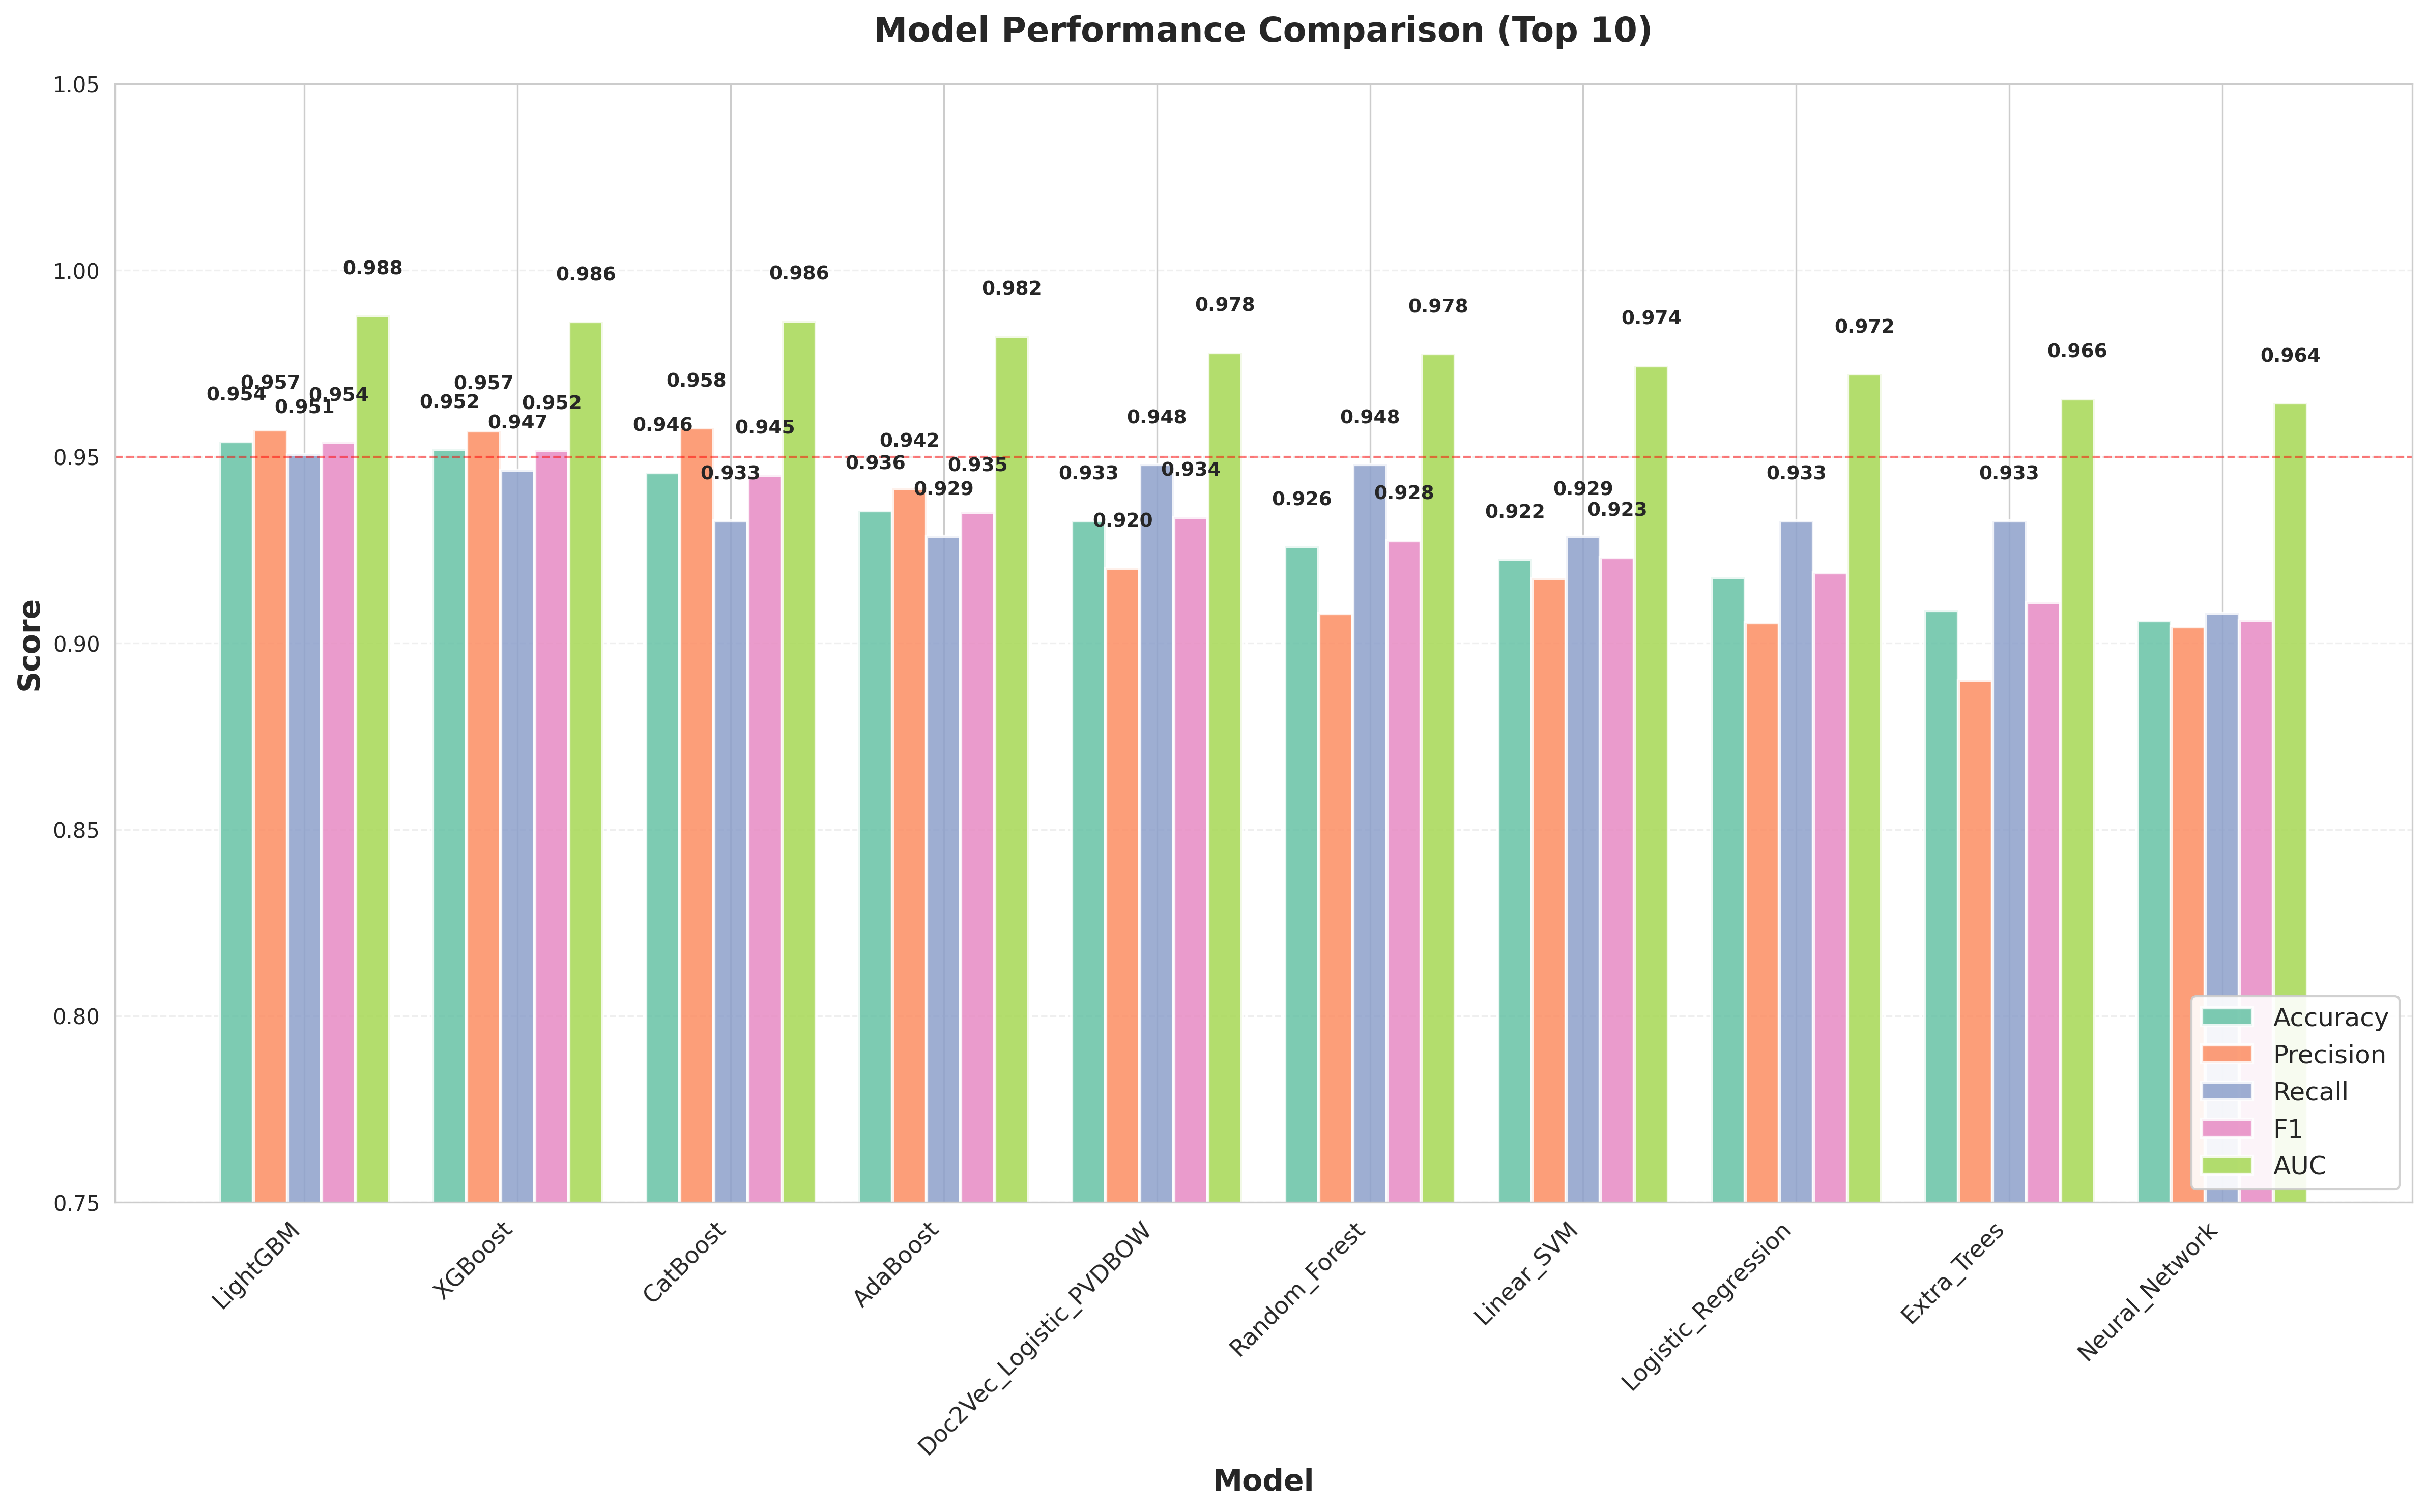
\includegraphics[width=0.85\linewidth]{experiment_figures/model_comparison.png}
    \caption{Comparison across all metrics for evaluated approaches.}
    \label{fig:comparison}
\end{figure}
\end{frame}

\begin{frame}{Additional Visualization}
\begin{figure}
    \centering
    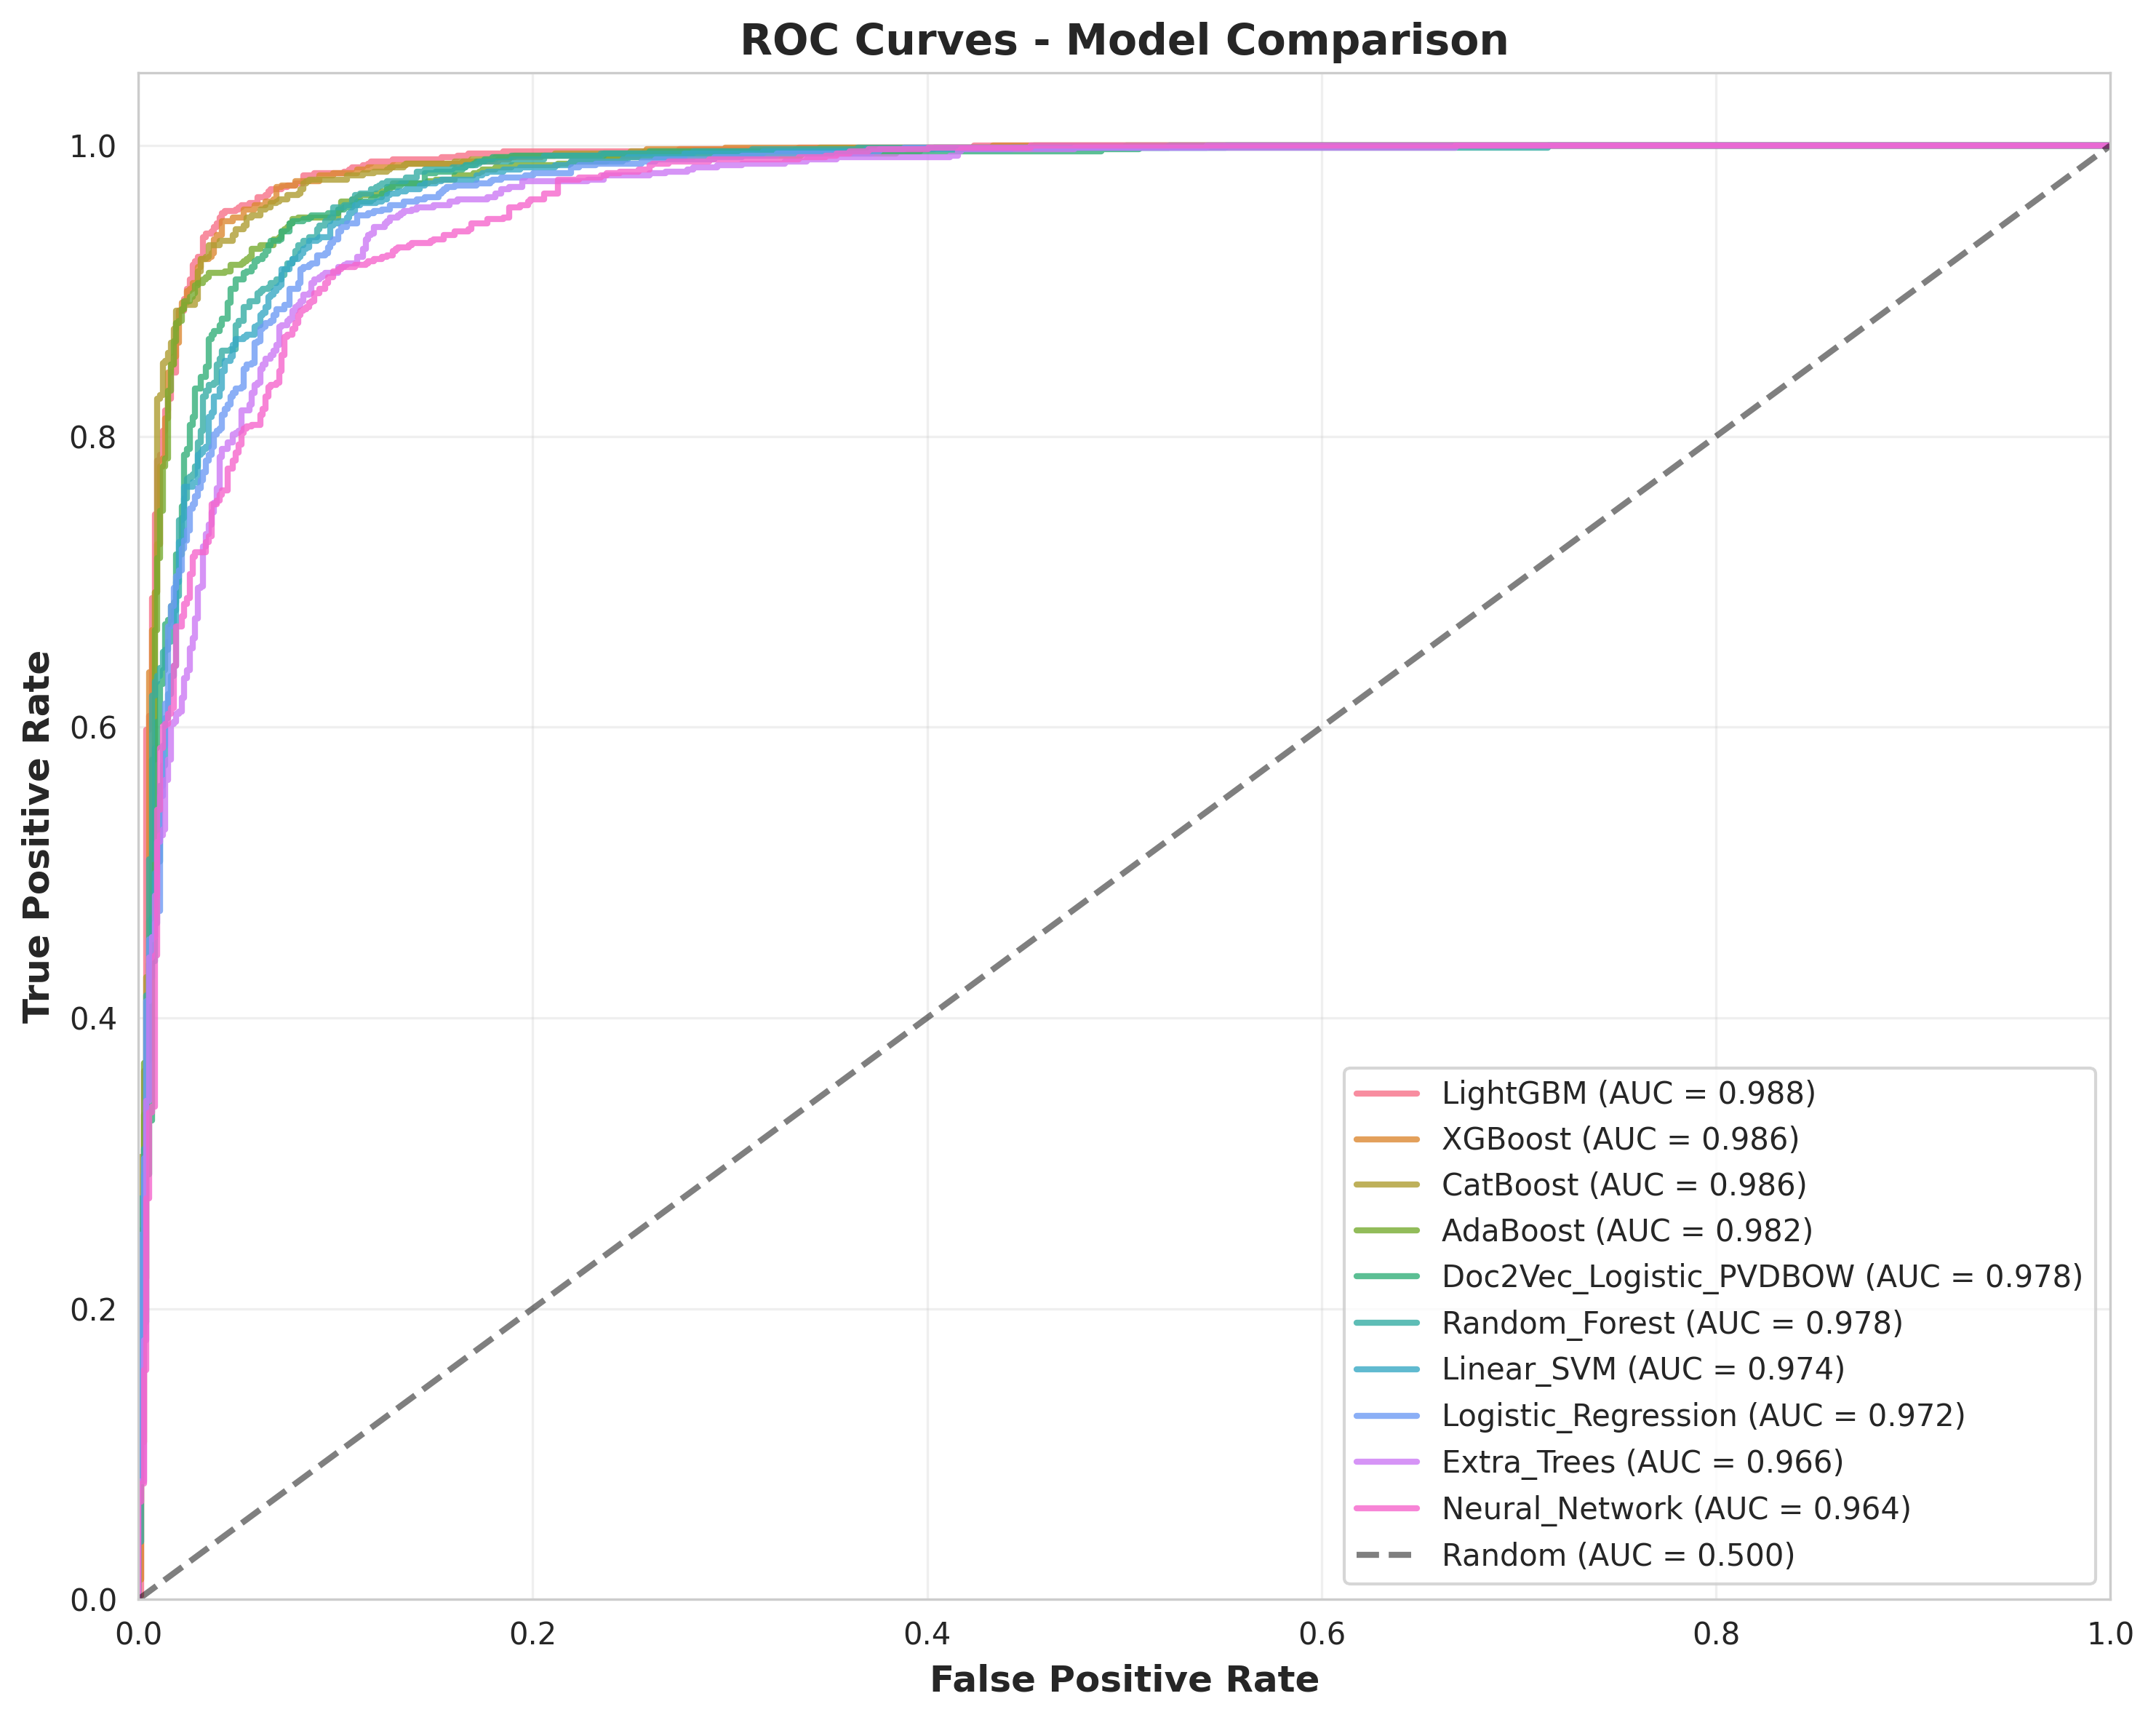
\includegraphics[width=0.65\linewidth]{experiment_figures/roc_curves.png}
    \caption{Additional analysis or visualization of results.}
    \label{fig:visualization}
\end{figure}
\end{frame}

\begin{frame}{Statistical Analysis}
\begin{itemize}
    \item Your best-performing approaches demonstrated clear superiority across multiple metrics.
    \item Statistical significance tests (e.g., t-tests, ANOVA, etc.) confirmed that these methods significantly outperform baseline approaches.
    \item Top approaches showed no statistically significant difference from each other ($p>0.XX$), though subtle performance variations were observed.
    \item All advanced methods significantly outperformed simpler baseline approaches ($p < 0.001$).
\end{itemize}
\end{frame}

\begin{frame}{Comparative Analysis}
\begin{table}[]
\centering
\small
\begin{tabular}{|l|c|c|c|}
\hline
\textbf{Approach} & \textbf{Metric 1} & \textbf{Metric 2} & \textbf{Metric 3} \\ \hline
\multicolumn{4}{|c|}{\cellcolor[HTML]{90EE90}\textbf{Category A Approaches}} \\ \hline
Approach A1 & \textbf{0.9539} & \textbf{0.9540} & \textbf{0.9879} \\ \hline
Approach A2 & 0.9517 & 0.9520 & 0.9862 \\ \hline
Approach A3 & 0.9451 & 0.9458 & 0.9865 \\ \hline
\multicolumn{4}{|c|}{\cellcolor[HTML]{FFD700}\textbf{Category B Approaches}} \\ \hline
Approach B1 & \textbf{0.9338} & \textbf{0.9328} & \textbf{0.9780} \\ \hline
Approach B2 & 0.8991 & 0.8944 & 0.9598 \\ \hline
Approach B3 & 0.8957 & 0.8923 & 0.9551 \\ \hline
\end{tabular}
\end{table}
\vspace{0.2cm}
\small
\textbf{Key Finding:} Category A consistently outperforms Category B, with best Category B approach still X\% below best Category A approach
\end{frame}

%==========================================================
% SECTION 3: DISCUSSION
%==========================================================

\begin{frame}{Detailed Analysis}
\begin{itemize}
    \item Extended analysis to test different combinations of approaches:
    \begin{itemize}
        \item Each variant paired with multiple configurations
        \item Total of X approach combinations tested
    \end{itemize}
    \item Key finding: Approach A + Technique X consistently outperformed Approach B + Technique X
    \item Best alternative: Approach B-Variant1 + Technique Y (Score: 0.9338)
    \item Still below best overall: Approach A1 + Technique X (Score: 0.9539)
\end{itemize}
\end{frame}

\begin{frame}{Performance Comparison Across Configurations}
\begin{table}[]
\centering
\small
\begin{tabular}{|l|c|c|c|c|c|}
\hline
\textbf{Feature Type} & \textbf{Config 1} & \textbf{Config 2} & \textbf{Config 3} & \textbf{Config 4} & \textbf{Config 5} \\ \hline
Feature A & 0.883 & 0.858 & 0.861 & 0.854 & 0.842 \\ \hline
Feature B & 0.864 & 0.845 & 0.832 & 0.839 & 0.833 \\ \hline
Feature C & \cellcolor[HTML]{90EE90}0.934 & 0.899 & 0.896 & 0.885 & 0.889 \\ \hline
Feature D & 0.885 & 0.844 & 0.841 & 0.844 & 0.823 \\ \hline
\rowcolor[HTML]{FFD700}
\textbf{Feature E} & \textbf{0.919} & \textbf{0.954} & \textbf{0.952} & \textbf{0.945} & \textbf{0.935} \\ \hline
\end{tabular}
\end{table}
\vspace{0.2cm}
\begin{itemize}
    \item \textbf{Observations:}
    \begin{itemize}
        \item Feature E dominates across \textbf{all} configuration types
        \item Feature C performs best among alternatives, especially with Config 1
        \item Configuration interactions vary significantly across feature types
        \item Different optimal pairings for different feature categories
    \end{itemize}
\end{itemize}
\end{frame}

\begin{frame}{Baseline Approach Performance}
\begin{itemize}
    \item Some simpler baseline approaches performed remarkably well despite their relative simplicity, achieving over 90\% performance and remaining competitive with more complex methods.
    \item This suggests that in certain feature spaces with proper preprocessing, simple decision boundaries can capture most of the relevant patterns.
    \item All advanced approaches significantly outperformed basic baselines with p-values below 0.001.
\end{itemize}
\end{frame}

\begin{frame}{Complex Model Performance}
\begin{itemize}
    \item \textbf{Model Architecture:} Description of your complex model structure
    \begin{itemize}
        \item Input layer configuration
        \begin{itemize}
            \scriptsize
            \item Variable input dimensions based on feature type
        \end{itemize}
        \item Hidden layer architecture (e.g., multiple layers with specific neuron counts)
        \item Activation functions, optimizer, and learning rate strategy
        \item Regularization and validation approach
    \end{itemize}
    \item \textbf{Performance:} Achieved X\% performance vs. baseline at Y\%
    \item \textbf{Data Limitations:} Dataset size or quality considerations that affected performance
    \item \textbf{Practical Implication:} Insights about when to use simpler vs. more complex approaches
\end{itemize}
\end{frame}

\begin{frame}{Alternative Approach Performance}
\begin{itemize}
    \item Alternative methods showed different performance characteristics, with X to Y percentage point differences compared to best approaches.
    \item These approaches make certain assumptions about the data structure that may not hold in all cases.
    \item Domain-specific characteristics can significantly impact the effectiveness of different method families.
    \item Statistical tests confirmed performance differences across approach categories.
\end{itemize}
\end{frame}

%==========================================================
% SECTION 4: CONCLUSIONS
%==========================================================

\begin{frame}{Conclusions and Recommendations}
\begin{itemize}
    \item Deploy best-performing approach for production system (X\% on metric 1, Y\% on metric 2)
    \item Use optimal feature representation for computational efficiency
    \item Adjust decision threshold based on application requirements:
    \begin{itemize}
        \item Higher recall to maximize coverage (at cost of precision)
        \item Higher precision to minimize false positives (at cost of recall)
    \end{itemize}
\end{itemize}

\end{frame}

\begin{frame}{Future Work}
\begin{itemize}
    \item Expand to additional domains or problem instances to verify generalization
    \item Develop extended classification system across broader categories
    \begin{itemize}
        \item Current state-of-the-art on related problems \cite{nguyen2023mimic}:
        \begin{itemize}
            \item Performance metric 1: X\% (Best Method)
            \item Performance metric 2: Y\% (Best Method)
        \end{itemize}
        \item Performance gap indicates opportunities for improvement
    \end{itemize}
    \item Incorporate additional data sources as they become available
    \item Define integration points within broader system architecture
\end{itemize}

\end{frame}

\end{document} 